\documentclass[12pt,a4paper]{report}

\usepackage[a4paper,top=1in,bottom=1in,left=1.25in,right=1in]{geometry}
\usepackage{setspace}
\usepackage{times}
\usepackage{array}
\usepackage{longtable}
\usepackage{booktabs}
\usepackage{titlesec}
\usepackage{tocloft}
\usepackage{graphicx}
\usepackage{tikz}
\usepackage{float}
\usepackage[section]{placeins}
\usepackage{hyperref}

\usetikzlibrary{arrows.meta,positioning,shapes.geometric}

\hypersetup{hidelinks}
\setstretch{1.5}
\setlength{\parindent}{0pt}
\setlength{\parskip}{6pt}
\setcounter{tocdepth}{3}

\titleformat{\chapter}[display]
  {\bfseries\Large}
  {\filcenter\MakeUppercase{\chaptertitlename} \thechapter}
  {1ex}
  {\centering\LARGE}

\newcommand{\HRule}{\rule{\linewidth}{0.6mm}}

\begin{document}

% Avoid duplicate hyperref page anchors on repeated titlepage page number 1.
\hypersetup{pageanchor=false}

% ------------------------------------------------------------------
% Title Page
% ------------------------------------------------------------------
\begin{titlepage}
\thispagestyle{empty}
\begin{center}

{\fontsize{18}{27}\selectfont\textbf{HEALTH CHAIN: INTEGRATING MYSQL}}\\[0.20cm]
{\fontsize{18}{27}\selectfont\textbf{WITH BLOCKCHAIN FOR RESILIENT}}\\[0.20cm]
{\fontsize{18}{27}\selectfont\textbf{HEALTHCARE SYSTEMS}}\\[1.00cm]

{\fontsize{14}{21}\selectfont\textbf{A PROJECT REPORT}}\\[0.55cm]
{\fontsize{14}{21}\selectfont\textbf{\textit{Submitted by}}}\\[0.65cm]

{\fontsize{16}{24}\selectfont\textbf{GAUTHAM R (720922104024)}}\\[0.28cm]
{\fontsize{16}{24}\selectfont\textbf{HARISH B (720922104029)}}\\[0.28cm]
{\fontsize{16}{24}\selectfont\textbf{KARTHICK R (720922104303)}}\\[0.28cm]
{\fontsize{16}{24}\selectfont\textbf{KISHORE R V (720922104305)}}\\[0.95cm]

{\fontsize{14}{21}\selectfont\textbf{\textit{in partial fulfillment for the award of the degree}}}\\[0.45cm]
{\fontsize{14}{21}\selectfont\textbf{\textit{of}}}\\[0.55cm]

{\fontsize{16}{24}\selectfont\textbf{BACHELOR OF ENGINEERING}}\\[0.35cm]
{\fontsize{14}{21}\selectfont\textbf{IN}}\\[0.35cm]
{\fontsize{14}{21}\selectfont\textbf{COMPUTER SCIENCE AND ENGINEERING}}\\[0.95cm]

{\fontsize{14}{21}\selectfont\textbf{DEPARTMENT OF COMPUTER SCIENCE AND ENGINEERING}}\\[0.25cm]
{\fontsize{14}{21}\selectfont\textbf{JCT COLLEGE OF ENGINEERING AND TECHNOLOGY}}\\[0.20cm]
{\fontsize{14}{21}\selectfont\textbf{Pichanur, Coimbatore}}\\[0.60cm]

{\fontsize{16}{24}\selectfont\textbf{ANNA UNIVERSITY : CHENNAI 600 025}}\\[0.70cm]

{\fontsize{14}{21}\selectfont\textbf{MARCH 2026}}

\end{center}
\end{titlepage}

% ------------------------------------------------------------------
% Bona Fide Certificate
% ------------------------------------------------------------------
\begin{titlepage}
\thispagestyle{empty}
\begin{center}
\vspace*{\fill}
{\fontsize{14}{21}\selectfont\textbf{2}}\\[0.20cm]
{\fontsize{14}{21}\selectfont\textbf{JCT COLLEGE OF ENGINEERING AND TECHNOLOGY}}\\[0.20cm]
{\fontsize{14}{21}\selectfont\textbf{(AUTONOMOUS)}}\\[0.20cm]
{\fontsize{14}{21}\selectfont\textbf{COIMBATORE - 641105}}\\[0.85cm]
{\fontsize{16}{24}\selectfont\textbf{BONA FIDE CERTIFICATE}}\\[0.65cm]

{\fontsize{14}{21}\selectfont
\begin{minipage}{0.90\textwidth}
\setlength{\parindent}{0pt}
Certified that this project report ``\textbf{HEALTH CHAIN: INTEGRATING MYSQL WITH BLOCKCHAIN FOR RESILIENT HEALTHCARE SYSTEMS}''
is the bonafide work of ``\textbf{GAUTHAM R, HARISH B, KARTHICK R, KISHORE R V}''
who carried out the project work under my supervision.
\\[0.45cm]
Submitted for the Viva Voce examination held on \rule{4cm}{0.4pt}
\end{minipage}}\\[1.4cm]
\end{center}

\begin{center}
\begin{minipage}{0.96\textwidth}
\begin{minipage}[t]{0.47\textwidth}
\textbf{SIGNATURE}\\[0.65cm]
\textbf{Dr. P. D. R. Vijayakumar}\\
\textbf{HEAD OF THE DEPARTMENT}\\[0.40cm]
\textbf{Department of Computer Science and Engineering}\\[0.35cm]
\textbf{JCT College of Engineering and Technology, Pichanur, Coimbatore - 641105}
\end{minipage}
\hfill
\begin{minipage}[t]{0.47\textwidth}
\textbf{SIGNATURE}\\[0.65cm]
\textbf{Ms. Annal Sheeba Rani E}\\
\textbf{SUPERVISOR}\\[0.35cm]
\textbf{Department of Computer Science and Engineering}\\[0.35cm]
\textbf{JCT College of Engineering and Technology, Pichanur, Coimbatore - 641105}
\end{minipage}
\end{minipage}
\end{center}

\vspace{0.9cm}
\begin{center}
\begin{minipage}{0.96\textwidth}
\begin{minipage}[t]{0.47\textwidth}
\textbf{INTERNAL EXAMINER}
\end{minipage}
\hfill
\begin{minipage}[t]{0.47\textwidth}
\textbf{EXTERNAL EXAMINER}
\end{minipage}
\end{minipage}
\end{center}

\vspace*{\fill}
\end{titlepage}

% ------------------------------------------------------------------
% Declaration
% ------------------------------------------------------------------
\begin{titlepage}
\thispagestyle{empty}
\begin{center}
{\fontsize{16}{24}\selectfont\textbf{DECLARATION}}\\[1.0cm]
\end{center}

\begin{minipage}{0.92\textwidth}
\setlength{\parindent}{0pt}
We hereby declare that this project report entitled
``\textbf{HEALTH CHAIN: INTEGRATING MYSQL WITH BLOCKCHAIN FOR RESILIENT HEALTHCARE SYSTEMS}''
is a record of original work carried out by us under the guidance of
\textbf{Ms. Annal Sheeba Rani E, Assistant Professor}, Department of Computer Science and Engineering,
JCT College of Engineering and Technology, Coimbatore, and has not formed the basis for the award
of any degree, diploma, associateship, fellowship, or any other similar title.
\end{minipage}

\vspace{1.2cm}

\begin{flushright}
\begin{tabular}{l}
\textbf{GAUTHAM R (720922104024)} \\
\textbf{HARISH B (720922104029)} \\
\textbf{KARTHICK R (720922104303)} \\
\textbf{KISHORE R V (720922104305)}
\end{tabular}
\end{flushright}

\vfill
\end{titlepage}

% Front matter page numbering in lower-case Roman numerals
\hypersetup{pageanchor=true}
\pagenumbering{roman}
\setcounter{page}{1}

% ------------------------------------------------------------------
% Abstract
% ------------------------------------------------------------------
\chapter*{ABSTRACT}
\addcontentsline{toc}{chapter}{ABSTRACT}

Health Chain is a full-stack Electronic Health Record system that combines a relational database workflow with an in-application blockchain ledger to provide tamper-evident clinical data management. The platform is designed to retain the practical benefits of a MySQL-based healthcare system while introducing a deterministic integrity layer that detects unauthorized modification of patient records.

The implemented architecture consists of a React frontend, an Express-based backend, a normalized MySQL schema, role-based access control with JWT, and a blockchain model persisted to JSON. During record creation, structured SOAP data is inserted transactionally into visit, vitals, diagnoses, and prescriptions tables. A deterministic clinical text representation is then hashed using SHA-256, and the hash is appended as a block linked to the previous block hash. Verification endpoints recompute the current hash from database state and compare it against the recorded blockchain hash to identify secure or tampered records.

The project additionally integrates operational healthcare requirements including appointment scheduling, doctor administration, patient timeline retrieval, and HIPAA-oriented audit logging. Security controls include password hashing, role-based authorization, optional transport security, and field-level encryption for sensitive profile attributes. Experimental walkthroughs confirm that while normal workflows remain responsive, direct database tampering is reliably detected by the blockchain verification pipeline. The result is a practical prototype that demonstrates how blockchain-assisted integrity can be integrated into conventional healthcare software without replacing the underlying relational model.

\chapter*{ACKNOWLEDGEMENT}
\addcontentsline{toc}{chapter}{ACKNOWLEDGEMENT}

We express our sincere gratitude to \textbf{Dr. P. D. R. Vijayakumar}, Head of the Department,
Department of Computer Science and Engineering, JCT College of Engineering and Technology,
for his encouragement and institutional support during this project.

We are deeply thankful to our guide, \textbf{Ms. Annal Sheeba Rani E, Assistant Professor},
for her valuable guidance, constructive feedback, and continuous motivation throughout the
development of this work.

We thank all faculty members, classmates, and well-wishers who contributed directly or indirectly
to the successful completion of this project report.

\newpage

% ------------------------------------------------------------------
% Table of Contents
% ------------------------------------------------------------------
\renewcommand{\contentsname}{TABLE OF CONTENTS}
\begin{center}
\textbf{CHAPTER NO. \hspace{2.2cm} TITLE \hspace{7.2cm} PAGE NO.}
\end{center}
\vspace{0.35cm}
\tableofcontents

\clearpage
\renewcommand{\listtablename}{LIST OF TABLES}
\begin{center}
\textbf{TABLE NO. \hspace{2.4cm} TITLE \hspace{7.1cm} PAGE NO.}
\end{center}
\vspace{0.35cm}
\listoftables
\addcontentsline{toc}{chapter}{LIST OF TABLES}

\clearpage
\renewcommand{\listfigurename}{LIST OF FIGURES}
\begin{center}
\textbf{FIGURE NO. \hspace{2.2cm} TITLE \hspace{7.0cm} PAGE NO.}
\end{center}
\vspace{0.35cm}
\listoffigures
\addcontentsline{toc}{chapter}{LIST OF FIGURES}

\clearpage
\chapter*{LIST OF SYMBOLS AND ABBREVIATIONS}
\addcontentsline{toc}{chapter}{LIST OF SYMBOLS AND ABBREVIATIONS}

\begin{longtable}{p{0.25\textwidth} p{0.67\textwidth}}
\toprule
\textbf{ABBREVIATION} & \textbf{EXPANSION} \\
\midrule
\endfirsthead
\toprule
\textbf{ABBREVIATION} & \textbf{EXPANSION} \\
\midrule
\endhead
\bottomrule
\endfoot

EHR & Electronic Health Records \\
RBAC & Role-Based Access Control \\
JWT & JSON Web Token \\
API & Application Programming Interface \\
SHA-256 & Secure Hash Algorithm 256-bit \\
HIPAA & Health Insurance Portability and Accountability Act \\
TLS & Transport Layer Security \\
CRUD & Create, Read, Update, Delete \\
DBMS & Database Management System \\
UI & User Interface \\

\end{longtable}

\newpage
\pagenumbering{arabic}
\setcounter{page}{1}

\chapter{INTRODUCTION}

\section{Background and Need}

Healthcare organizations depend on accurate and trustworthy records for diagnosis, treatment planning, legal compliance, insurance processing, and continuity of care. Most hospital information systems are built on centralized relational databases that provide efficient querying and structured storage. However, centralized storage alone does not inherently provide tamper evidence. If records are modified at the database level through unauthorized access, misconfiguration, or insider abuse, the system may not detect the change without an additional integrity mechanism.

Clinical records are highly sensitive and legally significant. A single altered diagnosis or prescription note can affect treatment decisions and patient safety. In this context, record integrity is not only a technical issue but also an ethical and regulatory requirement. This motivates a design where routine EHR operations remain practical while data integrity becomes independently verifiable.

Health Chain addresses this need by integrating MySQL with blockchain-style hash chaining. The project avoids replacing the relational model; instead, it introduces a complementary verification layer that marks each clinical record with a deterministic SHA-256 hash and stores it as a linked block. Any later mismatch between current record content and blockchain hash is treated as tampering.

\section{Problem Statement}

The central problem addressed in this project is:

\textit{How can a practical doctor-facing EHR platform preserve the efficiency of a normalized MySQL workflow while adding a robust and auditable mechanism to detect post-entry tampering of medical records?}

In routine healthcare systems, records are distributed across multiple normalized tables, and updates occur through user interfaces and backend APIs. This modularity improves maintainability but introduces challenges for integrity assurance:

\begin{enumerate}
\item record content is split across multiple tables and joins,
\item tampering may occur outside official application flows,
\item role-based access alone does not guarantee immutability,
\item audit logs help trace actions but do not independently prove record integrity.
\end{enumerate}

Hence, the requirement is to build a system where integrity can be verified deterministically at any time, with clear secure-versus-tampered outcomes.

\section{Project Objectives}

This project is developed with the following objectives:

\begin{enumerate}
\item Design a full-stack EHR workflow for doctors, patients, and administrators.
\item Implement transactional storage of SOAP records in normalized MySQL tables.
\item Generate deterministic SHA-256 hashes for clinical records.
\item Build an append-only blockchain ledger linked by previous-hash references.
\item Provide per-record and chain-level verification APIs for tamper detection.
\item Maintain HIPAA-oriented operational traceability using audit logging.
\item Support scheduling, dashboard analytics, and role-based access as real-world workflow features.
\end{enumerate}

\section{Scope and Boundaries}

\subsection{Included in Scope}

\begin{enumerate}
\item Web-based EHR workflow for patient records and appointments.
\item Role-based login for patient, doctor, and admin users.
\item Deterministic record hashing and blockchain block creation.
\item Verification APIs and blockchain explorer views.
\item Audit trail generation for key user actions.
\item Field-level encryption for selected profile attributes.
\end{enumerate}

\subsection{Out of Scope}

\begin{enumerate}
\item Public decentralized blockchain deployment.
\item Smart-contract execution on external chains.
\item Full production HIPAA certification process.
\item Integration with national EHR interoperability standards.
\item High-availability cloud deployment and auto-scaling.
\end{enumerate}

\section{Contributions of the Work}

\begin{enumerate}
\item A hybrid architecture that combines relational data handling with blockchain-based integrity checking.
\item Deterministic record serialization and hash generation strategy for reproducible verification.
\item Practical clinical workflow implementation with SOAP entry, timeline access, and scheduling.
\item End-to-end tamper detection capability with clear SECURE/TAMPERED outcomes.
\item Integrated compliance-minded features including audit logs and access controls.
\end{enumerate}

\begin{figure}[htbp]
\centering
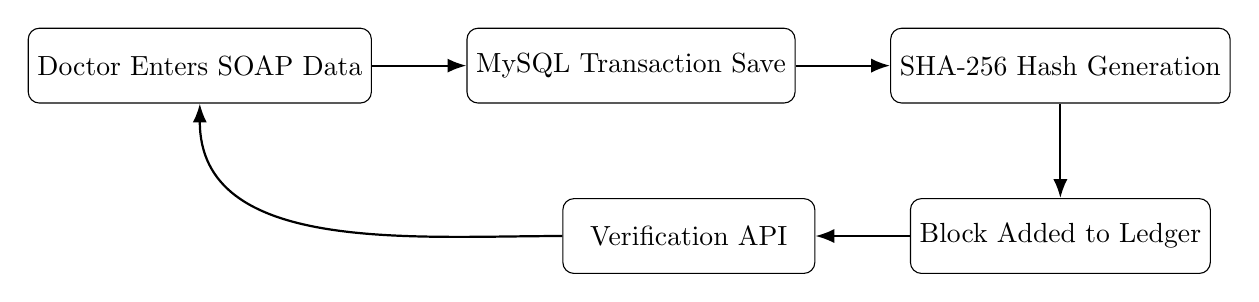
\begin{tikzpicture}[
node distance=1.2cm,
box/.style={draw, rounded corners, align=center, minimum width=3.2cm, minimum height=0.95cm},
arrow/.style={-{Latex[length=2.4mm]}, thick}
]
\node[box] (doctor) {Doctor Enters SOAP Data};
\node[box, right=of doctor] (db) {MySQL Transaction Save};
\node[box, right=of db] (hash) {SHA-256 Hash Generation};
\node[box, below=of hash] (block) {Block Added to Ledger};
\node[box, left=of block] (verify) {Verification API};

\draw[arrow] (doctor) -- (db);
\draw[arrow] (db) -- (hash);
\draw[arrow] (hash) -- (block);
\draw[arrow] (block) -- (verify);
\draw[arrow] (verify.west) to[out=180,in=-90] (doctor.south);
\end{tikzpicture}
\caption{Core integrity loop of the Health Chain system.}
\label{fig:healthchain-integrity-loop}
\end{figure}

\section{Report Organization}

The remainder of this report is structured as follows:

\begin{enumerate}
\item \textbf{Chapter 2} presents the literature survey and related work.
\item \textbf{Chapter 3} defines requirements, constraints, and technical specification.
\item \textbf{Chapter 4} explains architecture, modules, and system design.
\item \textbf{Chapter 5} details implementation methodology and core flows.
\item \textbf{Chapter 6} covers testing, validation, and observed results.
\item \textbf{Chapter 7} presents API design and end-to-end data flow analysis.
\item \textbf{Chapter 8} details security, privacy, and compliance-oriented controls.
\item \textbf{Chapter 9} explains deployment workflow, user operation guide, and viva preparation.
\item \textbf{Chapter 10} concludes with limitations and future enhancement directions.
\end{enumerate}

\chapter{LITERATURE SURVEY}

\section{Traditional EHR Systems and Integrity Challenges}

Conventional EHR systems are mostly built on centralized database architectures. They are optimized for structured storage, rapid retrieval, and complex clinical reporting through SQL. These systems support high transaction volumes and provide mature tooling for backup and recovery. Despite these strengths, many implementations rely on trust in access controls and administrative governance without embedding cryptographic tamper evidence in the data lifecycle.

Literature on healthcare security repeatedly identifies insider threat and privileged misuse as key risks. Even when role-based controls are present, database-level changes can be difficult to detect unless there is independent integrity instrumentation. This motivates cryptographic verification techniques that complement, rather than replace, mainstream EHR platforms.

\section{Blockchain in Healthcare Data Management}

Blockchain-inspired methods have been investigated for medical data provenance, consent traceability, and integrity assurance. Most studies emphasize immutability through linked blocks and cryptographic hashing, where any modification to prior data invalidates downstream chain consistency.

In practical healthcare software engineering, fully decentralized blockchain adoption often faces constraints such as operational complexity, cost, and integration friction with existing DBMS workflows. As a result, hybrid designs are increasingly explored: critical record fingerprints are anchored to a ledger while primary data remains in relational storage.

Health Chain follows this hybrid direction by storing complete clinical records in MySQL and preserving record fingerprints in a local chain. This strategy keeps query efficiency intact and introduces tamper detectability through deterministic hash comparison.

\section{Hash-Based Tamper Detection Approaches}

Cryptographic hash functions are widely used for integrity verification because small input changes produce large output differences. In medical record systems, deterministic record serialization is essential: identical logical content must always produce the same hash. If formatting is inconsistent, verification may fail even without tampering.

The reviewed approaches suggest that reliable tamper detection depends on:

\begin{enumerate}
\item stable canonical representation of record fields,
\item consistent ordering of serialized data,
\item secure hash function choice,
\item reliable mapping between stored records and integrity anchors.
\end{enumerate}

These principles are adopted in this project through a fixed SOAP text composition and SHA-256 hashing pipeline.

\section{Audit Logging and Compliance Perspective}

Healthcare regulation frameworks emphasize accountability and traceability. Audit logs capture who accessed what data and when actions occurred. However, logs alone do not prove that current record content is unchanged from original submission.

Therefore, best practice in security architecture combines event logging with cryptographic integrity checks. Health Chain reflects this integrated view by maintaining action-level audit trails alongside verification endpoints and chain validation routines.

\section{Research Gap and Motivation}

A clear practical gap exists between academic blockchain proposals and deployable student-level healthcare systems. Many studies discuss theoretical immutability but do not provide complete end-to-end implementations involving:

\begin{enumerate}
\item normalized healthcare schema,
\item transactional clinical inserts,
\item role-based APIs,
\item blockchain verification endpoints,
\item scheduler and dashboard workflows.
\end{enumerate}

This project is motivated by that implementation gap. It demonstrates a realistic, full-stack prototype where integrity verification is embedded into normal EHR operations rather than treated as a separate demonstration module.

\chapter{PROJECT REQUIREMENTS AND SPECIFICATION}

\section{Functional Requirements}

The system shall satisfy the following functional requirements:

\begin{enumerate}
\item Register and authenticate users with role-specific access.
\item Allow doctors to create full SOAP records for selected patients.
\item Persist visit data in normalized relational tables using transactions.
\item Generate deterministic SHA-256 hashes for every created visit record.
\item Append each record hash as a new block linked to prior blockchain state.
\item Provide record verification endpoint to classify SECURE or TAMPERED status.
\item Provide chain status endpoint for full blockchain validity checks.
\item Support patient profile retrieval and timeline visualization.
\item Support appointment booking with conflict detection and status updates.
\item Capture audit logs for key security and clinical actions.
\item Provide admin interfaces for doctor account management.
\end{enumerate}

\section{Non-Functional Requirements}

\begin{enumerate}
\item \textbf{Integrity}: deterministic and repeatable record verification.
\item \textbf{Security}: password hashing, role-based authorization, and token authentication.
\item \textbf{Reliability}: transactional inserts to avoid partial record state.
\item \textbf{Performance}: responsive API operations for standard clinic usage.
\item \textbf{Maintainability}: modular backend controllers and organized frontend components.
\item \textbf{Usability}: clear workflow for doctors and administrators.
\item \textbf{Auditability}: immutable-style evidence through chain and logs.
\end{enumerate}

\section{Input-Output Contracts}

\subsection*{Primary Inputs}

\begin{enumerate}
\item Authentication payloads (username, password).
\item Clinical record payloads (SOAP fields, vitals, severity, follow-up).
\item Scheduler payloads (patient, date, time, reason).
\item Verification requests (visit identifier).
\end{enumerate}

\subsection*{Primary Outputs}

\begin{enumerate}
\item JWT token and role metadata after login.
\item Persisted record identifier and blockchain hash after record creation.
\item Verification verdict for requested record.
\item Paginated datasets for patients, records, appointments, and audit logs.
\item Chain validity summary for blockchain monitoring.
\end{enumerate}

\section{Data Model Overview}

The database includes authentication tables, profile tables, visit tables, appointment table, and audit logs. Visits are normalized into visits, vitals, diagnoses, and prescriptions. This separation reduces redundancy and keeps data management structured, while the blockchain hash binds these distributed fields into a single integrity fingerprint.

\begin{table}[htbp]
\centering
\caption{Core data entities used in Health Chain.}
\label{tab:core-data-entities}
\begin{tabular}{p{0.24\textwidth} p{0.24\textwidth} p{0.42\textwidth}}
\toprule
\textbf{Entity} & \textbf{Category} & \textbf{Purpose} \\
\midrule
users & Authentication & Stores credentials and role mapping \\
patients, doctors & Profile & Stores domain-specific identity information \\
visits, vitals, diagnoses, prescriptions & Clinical & Stores normalized SOAP-linked encounter data \\
audit\_logs & Compliance & Stores action trace events \\
appointments & Scheduling & Stores doctor-patient slot planning records \\
blockchain\_data.json & Integrity & Stores linked block metadata and hashes \\
\bottomrule
\end{tabular}
\end{table}

\chapter{SYSTEM ARCHITECTURE AND DESIGN}

\section{High-Level Architecture}

The system is implemented as a three-tier architecture with a React-based client, Express API server, and MySQL database, augmented by a blockchain ledger file for integrity metadata. APIs act as the contract boundary between user interfaces and data services.

\begin{figure}[htbp]
\centering
\resizebox{0.92\textwidth}{!}{%
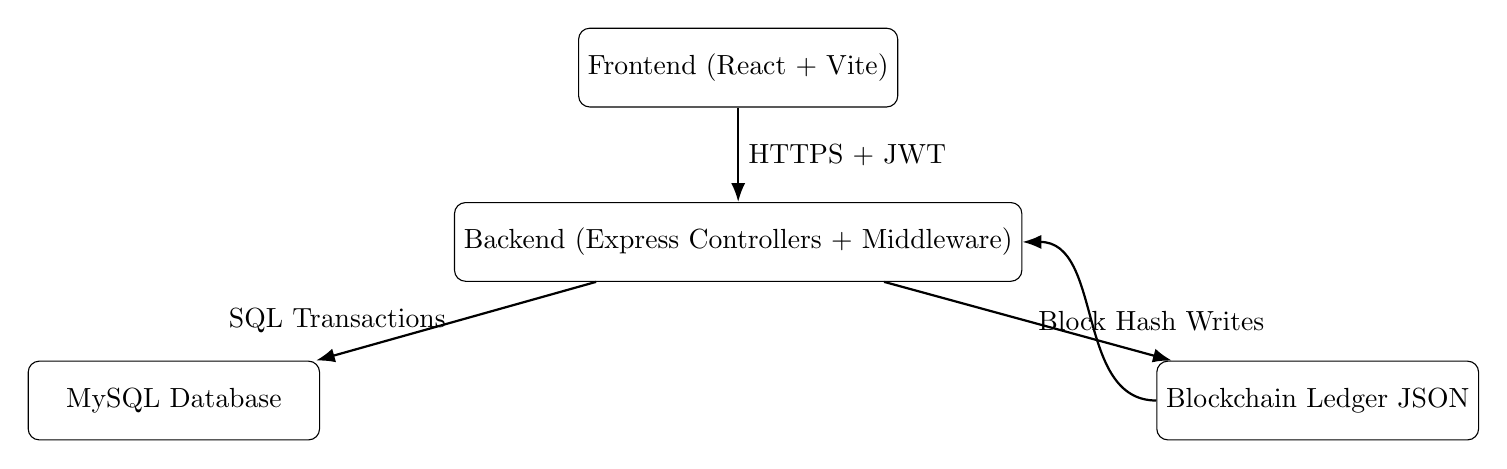
\begin{tikzpicture}[
node distance=1.2cm,
box/.style={draw, rounded corners, align=center, minimum width=3.7cm, minimum height=1.0cm},
arrow/.style={-{Latex[length=2.4mm]}, thick}
]
\node[box] (ui) {Frontend (React + Vite)};
\node[box, below=of ui] (api) {Backend (Express Controllers + Middleware)};
\node[box, below left=1.0cm and 1.7cm of api] (db) {MySQL Database};
\node[box, below right=1.0cm and 1.7cm of api] (bc) {Blockchain Ledger JSON};

\draw[arrow] (ui) -- node[right]{HTTPS + JWT} (api);
\draw[arrow] (api) -- node[left]{SQL Transactions} (db);
\draw[arrow] (api) -- node[right]{Block Hash Writes} (bc);
\draw[arrow] (bc.west) to[out=180,in=0] (api.east);
\end{tikzpicture}%
}
\caption{High-level architecture of the Health Chain platform.}
\label{fig:healthchain-architecture}
\end{figure}

\section{Backend Module Design}

The backend is organized into middleware, controllers, models, and utility layers.

\begin{enumerate}
\item \textbf{Middleware layer}: token verification and role authorization.
\item \textbf{Controller layer}: auth, records, appointments, dashboard, and admin flows.
\item \textbf{Model layer}: SQL transactions, record retrieval, chain operations.
\item \textbf{Utility layer}: hashing and sensitive-field encryption support.
\end{enumerate}

This separation improves maintainability and allows integrity logic to remain explicit in record workflows.

\section{Record Creation and Verification Flow}

Figure~\ref{fig:record-create-verify-flow} presents the operational data flow for record creation and verification.

\begin{figure}[htbp]
\centering
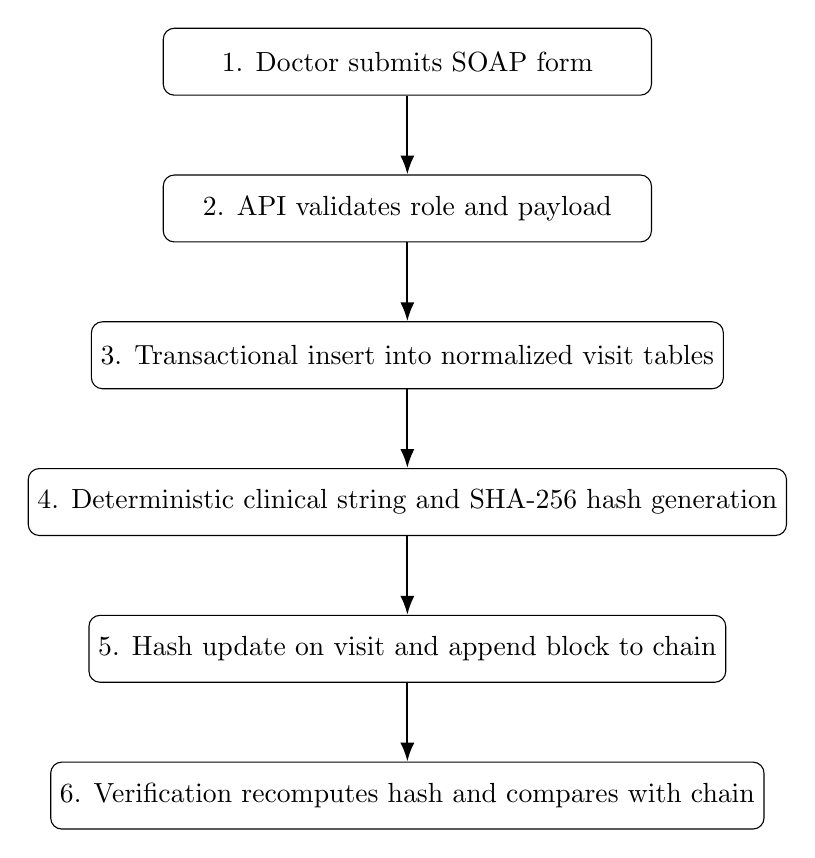
\begin{tikzpicture}[
node distance=1.0cm,
flow/.style={draw, rounded corners, align=center, minimum width=6.2cm, minimum height=0.85cm},
arrow/.style={-{Latex[length=2.4mm]}, thick}
]
\node[flow] (f1) {1. Doctor submits SOAP form};
\node[flow, below=of f1] (f2) {2. API validates role and payload};
\node[flow, below=of f2] (f3) {3. Transactional insert into normalized visit tables};
\node[flow, below=of f3] (f4) {4. Deterministic clinical string and SHA-256 hash generation};
\node[flow, below=of f4] (f5) {5. Hash update on visit and append block to chain};
\node[flow, below=of f5] (f6) {6. Verification recomputes hash and compares with chain};

\draw[arrow] (f1) -- (f2);
\draw[arrow] (f2) -- (f3);
\draw[arrow] (f3) -- (f4);
\draw[arrow] (f4) -- (f5);
\draw[arrow] (f5) -- (f6);
\end{tikzpicture}
\caption{Clinical record creation and integrity verification workflow.}
\label{fig:record-create-verify-flow}
\end{figure}

\section{Security and Compliance Design}

Security design includes authentication, authorization, data protection, and accountability.

\begin{enumerate}
\item Passwords are stored using bcrypt hashes.
\item JWT tokens carry user identity and role claims.
\item Role checks are enforced per API endpoint.
\item Sensitive profile fields can be encrypted at rest.
\item Audit logs record critical actions including record creation and verification.
\end{enumerate}

\chapter{DATABASE DESIGN AND DATA FLOW}

\section{Database Overview}

The database is the central operational backbone of HealthChain Bridge because all critical workflows depend on reliable persisted state: authentication, patient profile access, clinical record creation, appointment scheduling, integrity verification, and compliance logging.

The design follows a hybrid approach:

\begin{enumerate}
\item \textbf{Relational storage (MySQL):} canonical healthcare entities and transactional operations.
\item \textbf{Integrity ledger (JSON blockchain):} tamper-evident hash anchoring linked to record identifiers.
\end{enumerate}

This ensures that day-to-day clinical operations keep SQL efficiency while integrity checks remain independently verifiable.

In practical terms, this hybrid choice addresses a common healthcare software gap. Traditional systems are strong at structured retrieval but weak at proving post-write immutability. Pure decentralized blockchain systems provide stronger immutability semantics but introduce operational complexity for normal hospital or clinic workflows. HealthChain Bridge therefore takes a middle path: keep high-usability transactional storage in MySQL and attach cryptographic trust signals through a deterministic ledger layer.

From an engineering perspective, this also improves maintainability. Database administrators can continue using familiar SQL tooling for backup, migration, and query optimization, while integrity validation can evolve independently as a service concern. This separation is important for final-year systems because it demonstrates both conceptual correctness and implementation pragmatism.

\section{Core Relational Schema Design}

The schema is mapped to real system workflows rather than abstract entities. Major tables include:

\begin{enumerate}
\item \texttt{users}: authentication identity and role.
\item \texttt{patients} and \texttt{doctors}: profile-level role extensions.
\item \texttt{visits}, \texttt{vitals}, \texttt{diagnoses}, \texttt{prescriptions}: normalized SOAP persistence.
\item \texttt{appointments}: scheduling lifecycle.
\item \texttt{audit\_logs}: compliance traceability.
\end{enumerate}

The normalization strategy supports clean joins for patient timeline retrieval and prevents update anomalies in clinical detail storage.

Another design objective was to preserve semantic clarity between encounter-level and measurement-level data. For example, a visit represents the clinical context (who, when, why), while vitals and diagnosis represent structured observations linked to that context. This mapping avoids overloading a single table with mixed concerns and helps both analytics and audit review workflows.

\section{Transactional Database Reliability}

Clinical record insertion is treated as an atomic multi-table operation. The backend creates visit, vitals, diagnosis, and prescription rows inside one transaction, so no partial record state is committed.

This choice improves both clinical reliability and engineering correctness:

\begin{enumerate}
\item failed intermediate write $\Rightarrow$ full rollback,
\item successful commit $\Rightarrow$ complete and query-consistent record set.
\end{enumerate}

This transactional behavior directly supports integrity validation quality. If record fragments were partially committed, a later verification operation could fail for the wrong reason (incomplete data rather than tampering). By enforcing atomic writes, the project ensures that mismatch signals remain meaningful and interpretable.

\section{Database Relationship and Access Path}

Role-specific query paths are intentionally separated:

\begin{enumerate}
\item doctors/admins can query broader patient and operational datasets,
\item patient access is constrained to self-scoped records and status views,
\item admin modules use dedicated joins for doctor account management.
\end{enumerate}

This creates predictable access boundaries at query level, not only at UI level.

\begin{figure}[htbp]
\centering
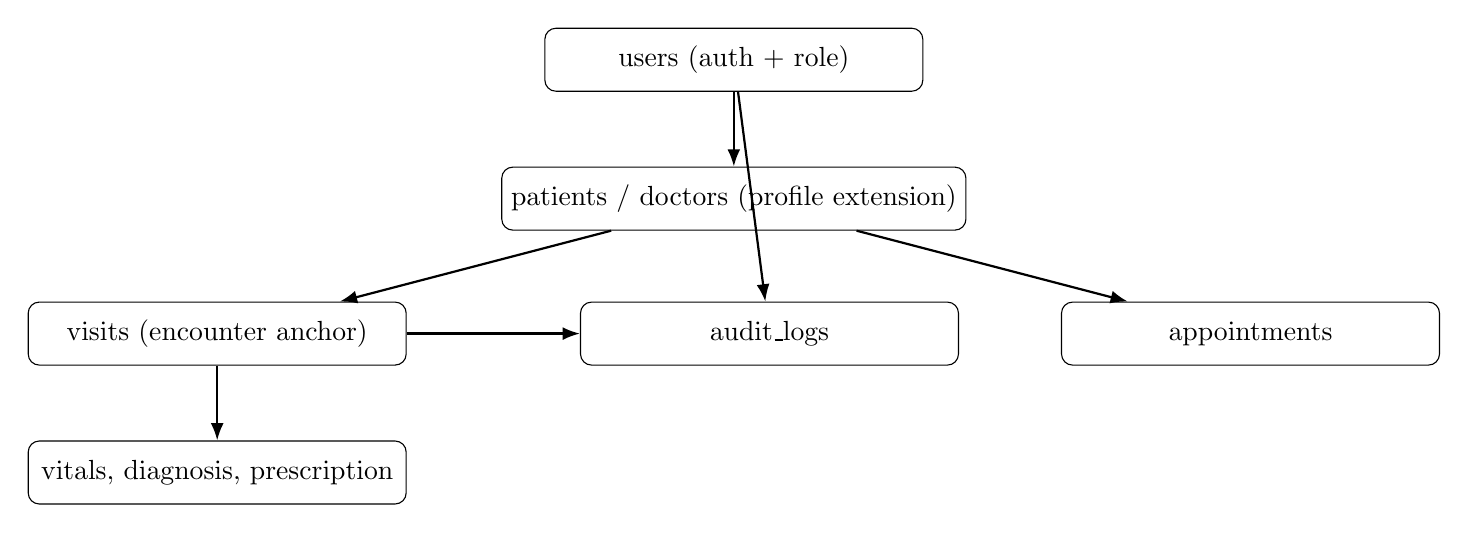
\begin{tikzpicture}[
node distance=0.95cm,
tbl/.style={draw, rounded corners, align=center, minimum width=4.8cm, minimum height=0.8cm},
arrow/.style={-{Latex[length=2.2mm]}, thick}
]
\node[tbl] (u) {users (auth + role)};
\node[tbl, below=of u] (p) {patients / doctors (profile extension)};
\node[tbl, below left=0.9cm and 1.2cm of p] (v) {visits (encounter anchor)};
\node[tbl, below=of v] (c1) {vitals, diagnosis, prescription};
\node[tbl, below right=0.9cm and 1.2cm of p] (a) {appointments};
\node[tbl, right=2.2cm of v] (l) {audit\_logs};

\draw[arrow] (u) -- (p);
\draw[arrow] (p) -- (v);
\draw[arrow] (v) -- (c1);
\draw[arrow] (p) -- (a);
\draw[arrow] (u) -- (l);
\draw[arrow] (v) -- (l);
\end{tikzpicture}
\caption{Simplified relational dependency view for HealthChain operational tables.}
\label{fig:db-dependency-view}
\end{figure}

\begin{table}[htbp]
\centering
\caption{Core tables used in HealthChain application database.}
\label{tab:core-database-tables}
\begin{tabular}{p{0.28\textwidth} p{0.20\textwidth} p{0.42\textwidth}}
\toprule
\textbf{Table} & \textbf{Type} & \textbf{Role in Workflow} \\
\midrule
users & Auth core & Login identity, hashed password, role claims \\
patients & Profile & Patient demographic and medical profile context \\
doctors & Profile & Clinician identity and specialty mapping \\
visits & Clinical core & Encounter-level SOAP anchor and hash reference \\
vitals & Clinical detail & Objective measurements linked to visit \\
diagnoses & Clinical detail & Assessment and severity linked to visit \\
prescriptions & Clinical detail & Plan/medication instructions linked to visit \\
appointments & Scheduling & Date/time/status-based consultation planning \\
audit\_logs & Compliance & Immutable action-level operational trace \\
\bottomrule
\end{tabular}
\end{table}

\section{Data Flow from Record Creation to Verification}

The key database-centric flow in this project is the lifecycle from record insert to tamper validation:

\begin{enumerate}
\item write normalized SOAP tables transactionally,
\item build deterministic canonical SOAP string,
\item generate SHA-256 hash and store in relational record,
\item append hash fingerprint to blockchain ledger with previous-hash link,
\item on verification, reconstruct current DB content and compare hashes.
\end{enumerate}

This ensures database state and ledger state remain cross-checkable at any point in time.

\begin{figure}[H]
\centering
\fbox{\begin{minipage}[c][3.5cm][c]{0.88\textwidth}
\centering
\textbf{Placeholder: MySQL Schema Screenshot}\\[0.25cm]
Add: database schema/ER view showing users, patients, doctors, visits, vitals, diagnoses, prescriptions, appointments, audit\_logs.
\end{minipage}}
\caption{Suggested screenshot for Chapter 5: relational schema evidence.}
\label{fig:placeholder-db-schema}
\end{figure}

\section{Database and Data-Flow Summary}

Chapter 5 established the project as a database-grounded healthcare system where trust is strengthened through cryptographic verification. The next chapter focuses on software engineering implementation workflows that operationalize these data and integrity designs in production-style modules.

\section{Implementation Flow Diagram}

\begin{figure}[htbp]
\centering
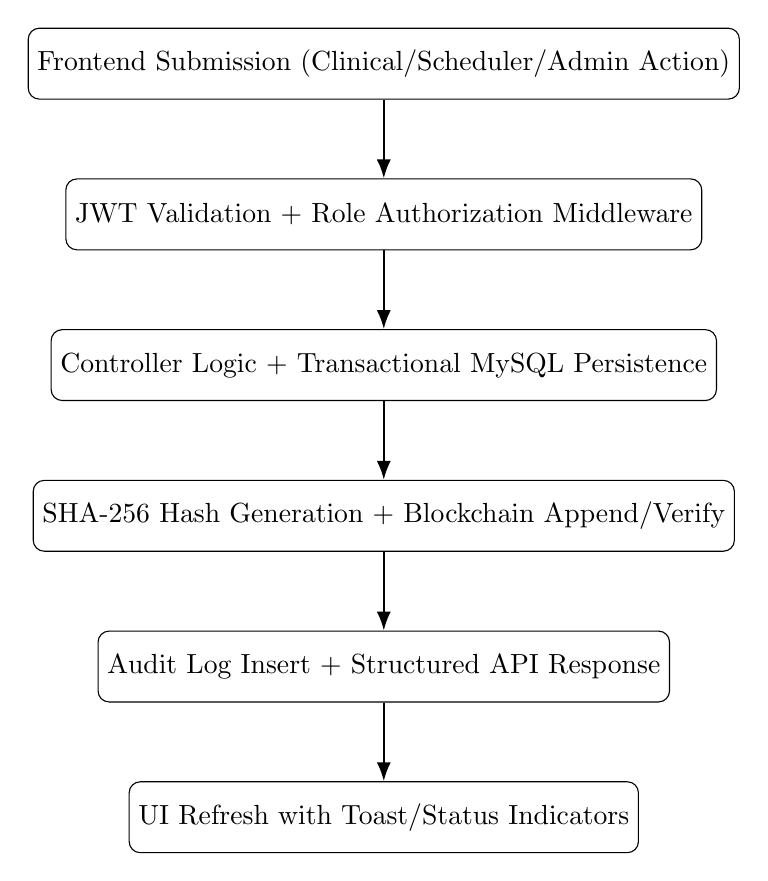
\begin{tikzpicture}[
node distance=1.0cm,
flow/.style={draw, rounded corners, align=center, minimum width=6.0cm, minimum height=0.9cm},
arrow/.style={-{Latex[length=2.4mm]}, thick}
]
\node[flow] (i1) {Frontend Submission (Clinical/Scheduler/Admin Action)};
\node[flow, below=of i1] (i2) {JWT Validation + Role Authorization Middleware};
\node[flow, below=of i2] (i3) {Controller Logic + Transactional MySQL Persistence};
\node[flow, below=of i3] (i4) {SHA-256 Hash Generation + Blockchain Append/Verify};
\node[flow, below=of i4] (i5) {Audit Log Insert + Structured API Response};
\node[flow, below=of i5] (i6) {UI Refresh with Toast/Status Indicators};

\draw[arrow] (i1) -- (i2);
\draw[arrow] (i2) -- (i3);
\draw[arrow] (i3) -- (i4);
\draw[arrow] (i4) -- (i5);
\draw[arrow] (i5) -- (i6);
\end{tikzpicture}
\caption{End-to-end implementation flow from user action to blockchain-backed response.}
\label{fig:implementation-flow}
\end{figure}

\chapter{SOFTWARE ENGINEERING IMPLEMENTATION WORKFLOW}

\section{Engineering Environment and Stack Composition}

After establishing data architecture, the implementation was engineered as a modular full-stack workflow where each layer has a clear responsibility.

\begin{enumerate}
\item \textbf{Client engineering:} React + Vite route-based UI with role-aware navigation and reusable components.
\item \textbf{API engineering:} Express controllers with middleware-driven security and validation.
\item \textbf{Model engineering:} encapsulated data and blockchain operations to avoid business logic duplication.
\item \textbf{Utility engineering:} isolated hashing and encryption helpers for deterministic reuse.
\end{enumerate}

The engineering approach intentionally favors separation of concerns over shortcut coding patterns. UI pages are organized by role and workflow, controllers are scoped by business capability, and shared helpers reduce repeated crypto/security logic. This structure was chosen to make debugging, testing, and viva explanation easier, since each module has a single dominant responsibility.

\section{Backend Engineering Workflow}

The backend implementation follows a clean request pipeline:

\begin{enumerate}
\item route mapping,
\item token and role middleware,
\item controller orchestration,
\item model/database execution,
\item audit and response emission.
\end{enumerate}

This pattern improves maintainability because each layer is testable and change-scoped.

A key implementation quality point is that policy checks happen before business execution. In other words, authentication and authorization failures are resolved at middleware stage, not deep inside controller branches. This reduces hidden edge cases and makes negative-path behavior easier to reason about.

\subsection{Controller-Oriented Business Modules}

The implementation is engineered as domain modules rather than one large controller:

\begin{enumerate}
\item authentication and account flow,
\item clinical record management and verification,
\item appointment scheduling and conflict control,
\item dashboard analytics aggregation,
\item admin provisioning workflows.
\end{enumerate}

This modularity reduces coupling and improves feature extensibility.

\subsection{Codebase Organization and Reuse Strategy}

Reusable components and utilities are treated as first-class engineering assets in the implementation. On the frontend, shared elements such as patient search, pagination, records cards, and layout controls reduce UI duplication. On the backend, utility abstractions for hashing, encryption, and role middleware provide consistent behavior across route families.

This reuse strategy reduces regression risk. When security or validation behavior is updated in one shared module, all dependent routes or pages inherit the improvement without repeated edits.

\subsection{Reliability and Consistency Engineering}

Reliability is enforced through transactional persistence and deterministic integrity operations. Critical write workflows are atomic, and integrity artifacts are generated from canonical serialized input, making verification behavior reproducible across environments.

\subsection{Failure Handling and Recovery Paths}

Implementation quality is also reflected in predictable failure handling:

\begin{enumerate}
\item validation errors return explicit client-consumable messages,
\item conflict scenarios use semantic HTTP 409 responses,
\item unauthorized paths terminate early with 403 responses,
\item verification failures return safe status classifications instead of silent success.
\end{enumerate}

These choices improve operational reliability and reduce ambiguity during demonstrations and testing.

\section{Cross-Layer Integration Flow}

The project engineering focus is not only feature presence, but integration consistency across modules:

\begin{enumerate}
\item frontend submits authenticated payloads,
\item middleware enforces access policy,
\item controllers orchestrate model operations,
\item relational and blockchain states are updated coherently,
\item audit logging preserves post-action traceability.
\end{enumerate}

\begin{table}[htbp]
\centering
\caption{Engineering module responsibilities across implementation layers.}
\label{tab:engineering-module-map}
\begin{tabular}{p{0.30\textwidth} p{0.22\textwidth} p{0.38\textwidth}}
\toprule
\textbf{Module} & \textbf{Layer} & \textbf{Engineering Role} \\
\midrule
apiRoutes + middleware & Integration layer & Route binding, JWT validation, RBAC policy \\
authController & Business layer & Account lifecycle and token issuance \\
recordController & Business layer & Multi-table clinical flow + verify orchestration \\
appointmentController & Business layer & Conflict-safe scheduling lifecycle \\
Records model & Data layer & Transactional DB write/read encapsulation \\
Blockchain model & Integrity layer & Linked-block persistence and validation \\
AuditLog model & Compliance layer & Action trace persistence for accountability \\
\bottomrule
\end{tabular}
\end{table}

\begin{figure}[htbp]
\centering
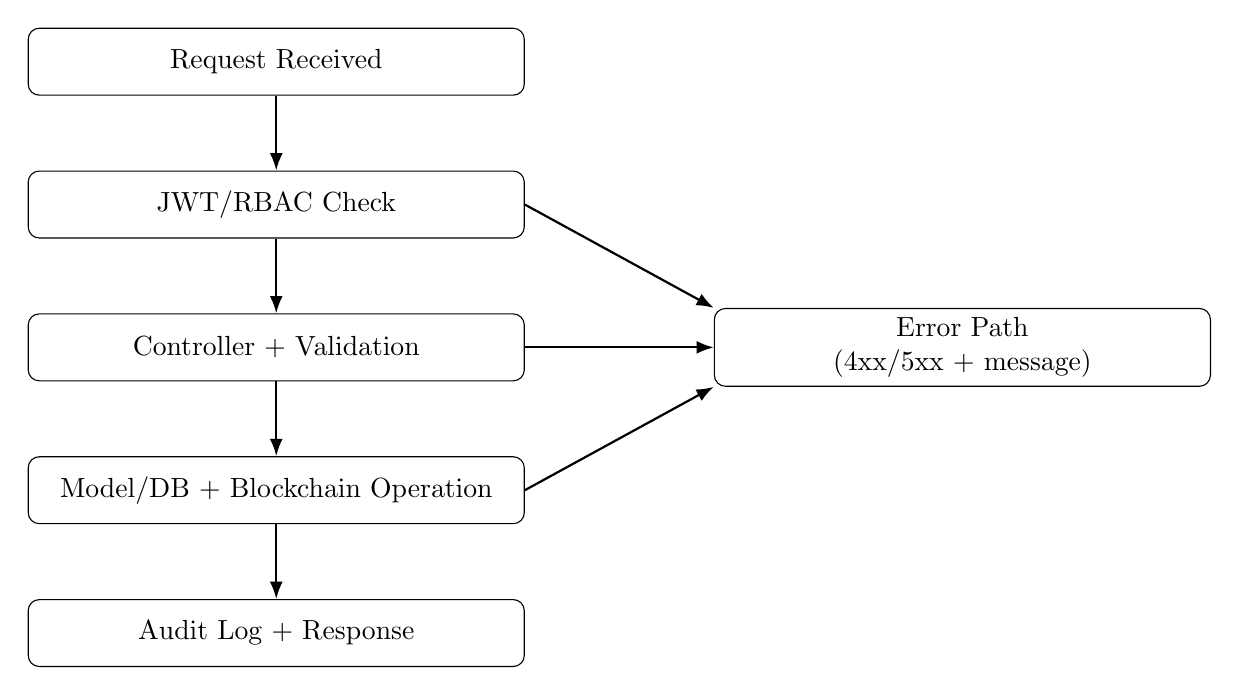
\begin{tikzpicture}[
node distance=0.95cm,
flowbox/.style={draw, rounded corners, align=center, minimum width=6.3cm, minimum height=0.85cm},
arrow/.style={-{Latex[length=2.2mm]}, thick}
]
\node[flowbox] (s1) {Request Received};
\node[flowbox, below=of s1] (s2) {JWT/RBAC Check};
\node[flowbox, below=of s2] (s3) {Controller + Validation};
\node[flowbox, below=of s3] (s4) {Model/DB + Blockchain Operation};
\node[flowbox, below=of s4] (s5) {Audit Log + Response};
\node[flowbox, right=2.4cm of s3] (e1) {Error Path\\(4xx/5xx + message)};

\draw[arrow] (s1) -- (s2);
\draw[arrow] (s2) -- (s3);
\draw[arrow] (s3) -- (s4);
\draw[arrow] (s4) -- (s5);
\draw[arrow] (s2.east) -- (e1.north west);
\draw[arrow] (s3.east) -- (e1.west);
\draw[arrow] (s4.east) -- (e1.south west);
\end{tikzpicture}
\caption{Engineering request lifecycle with normal and failure branches.}
\label{fig:engineering-request-lifecycle}
\end{figure}

\section{Engineering Discussion}

The implementation demonstrates practical software engineering progression from architecture to reliable workflows. Frontend concerns were established in earlier chapters; this chapter emphasized backend orchestration, module separation, integration quality, and reliability choices that make the system maintainable and extensible.

\begin{figure}[H]
\centering
\fbox{\begin{minipage}[c][3.5cm][c]{0.88\textwidth}
\centering
\textbf{Placeholder: Backend Folder Structure Screenshot}\\[0.25cm]
Add: server/src tree showing controllers, middleware, models, routes, utils to evidence modular engineering.
\end{minipage}}
\caption{Suggested screenshot for Chapter 6: modular backend organization evidence.}
\label{fig:placeholder-backend-structure}
\end{figure}

\chapter{LOGIC DESIGN AND INTEGRITY ENGINE}

\section{Chapter Purpose and Logic Scope}

This chapter explains the core logic that gives HealthChain Bridge its technical value beyond interface and database implementation. While earlier chapters covered data structures and software engineering workflow, this chapter focuses on decision rules and algorithmic behavior: how record content is canonicalized, how hashes are generated, how blockchain linkage is created, how verification verdicts are computed, and how scheduling and role-access decisions are made.

The main idea is that trust in records should not depend only on access control; it should be computable and re-checkable through deterministic logic.

\section{Deterministic SOAP Canonicalization Logic}

The integrity pipeline begins by transforming clinical record content into a canonical string representation. This step is crucial because hash verification is only meaningful when the same logical record always produces the same input string.

The implemented canonical pattern follows the SOAP structure:

\begin{enumerate}
\item Subjective line (chief complaint and relevant narrative),
\item Objective line (vitals in normalized order),
\item Assessment line (diagnosis/severity context),
\item Plan line (prescription and follow-up instruction).
\end{enumerate}

Whitespace trimming and stable field ordering are enforced to avoid accidental hash drift caused by formatting differences. This means comparison failures are more likely to indicate genuine content changes rather than serialization noise.

\section{Hash Generation and Block Anchoring Logic}

After canonicalization, the system computes a SHA-256 digest and stores it as the record fingerprint. A new blockchain block is then created with index, timestamp, record id, data hash, previous hash, and current hash.

The block hash follows a deterministic composition of block fields. Conceptually:

$$
\mathrm{currentHash} = H(\mathrm{index} \parallel \mathrm{timestamp} \parallel \mathrm{recordId} \parallel \mathrm{dataHash} \parallel \mathrm{previousHash})
$$

where $H$ is SHA-256 and $\parallel$ denotes concatenation in fixed order.

This chaining ensures that modifying one block affects all downstream hash relationships, making tampering detectable.

\section{Verification Decision Engine}

The verification logic is a deterministic decision engine rather than a heuristic check. Its runtime sequence is:

\begin{enumerate}
\item fetch relational record components for the target visit,
\item rebuild canonical SOAP string using the same formatting logic,
\item recompute SHA-256 hash,
\item fetch blockchain-stored hash for the same record id,
\item compare recomputed hash with anchored hash,
\item emit verdict: \texttt{SECURE} or \texttt{TAMPERED}.
\end{enumerate}

Decision rule:

$$
\mathrm{status} =
\left\{
\begin{array}{ll}
\mathrm{SECURE}, & \mathrm{if}\ h_{db} = h_{chain} \\
\mathrm{TAMPERED}, & \mathrm{if}\ h_{db} \neq h_{chain}
\end{array}
\right.
$$

This binary decision model provides clear interpretation for users and reviewers.

\begin{figure}[htbp]
\centering
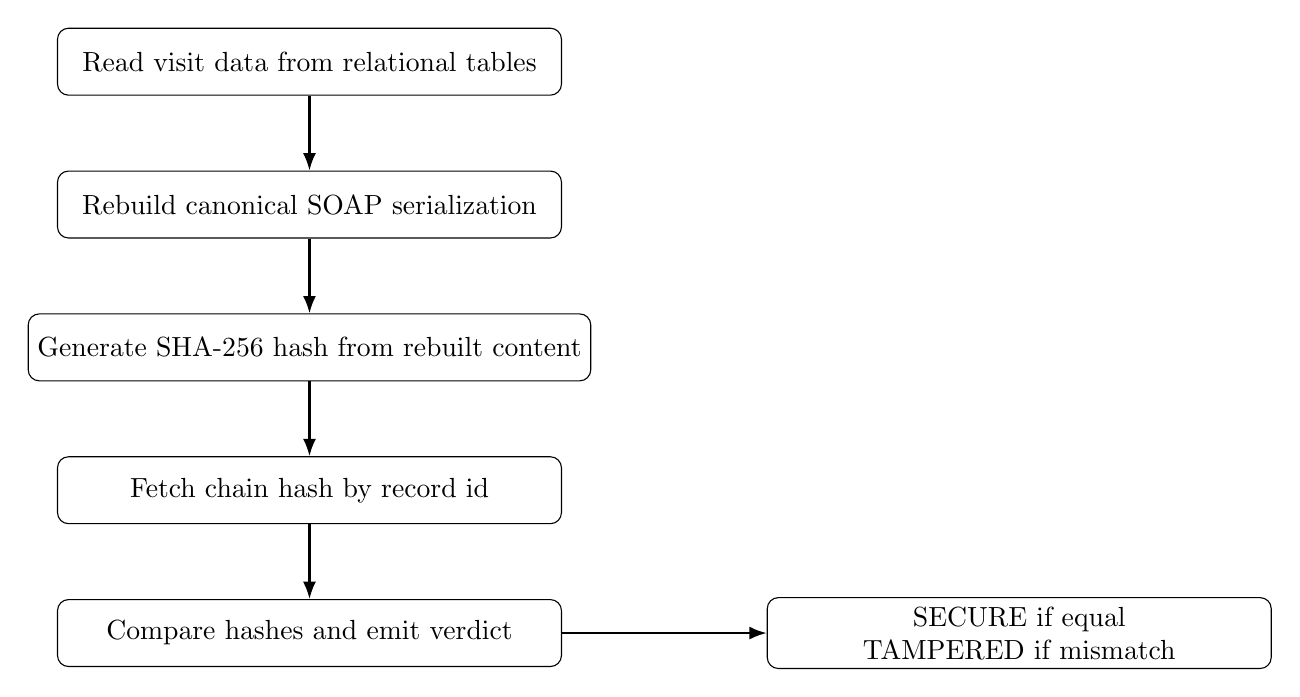
\begin{tikzpicture}[
node distance=0.95cm,
logicbox/.style={draw, rounded corners, align=center, minimum width=6.4cm, minimum height=0.85cm},
arrow/.style={-{Latex[length=2.2mm]}, thick}
]
\node[logicbox] (v1) {Read visit data from relational tables};
\node[logicbox, below=of v1] (v2) {Rebuild canonical SOAP serialization};
\node[logicbox, below=of v2] (v3) {Generate SHA-256 hash from rebuilt content};
\node[logicbox, below=of v3] (v4) {Fetch chain hash by record id};
\node[logicbox, below=of v4] (v5) {Compare hashes and emit verdict};
\node[logicbox, right=2.6cm of v5] (v6) {SECURE if equal\\TAMPERED if mismatch};

\draw[arrow] (v1) -- (v2);
\draw[arrow] (v2) -- (v3);
\draw[arrow] (v3) -- (v4);
\draw[arrow] (v4) -- (v5);
\draw[arrow] (v5) -- (v6);
\end{tikzpicture}
\caption{Verification decision flow used by the integrity engine.}
\label{fig:verification-decision-flow}
\end{figure}

\section{Role and Access Decision Logic}

Role handling is implemented as a two-stage policy decision:

\begin{enumerate}
\item identity validation (JWT token parsing and signature check),
\item route authorization (allowed role set per endpoint).
\end{enumerate}

The decision is fail-closed: when token validation fails or role is outside allowed set, request execution is terminated before business logic. This prevents unauthorized paths from reaching sensitive operations.

\section{Scheduler Conflict Decision Logic}

Appointment creation uses deterministic overlap rules to avoid double-booking behavior for doctors. On each new request, the system checks nearby timeslots in the same date window for conflict. If overlap exists within configured tolerance, the booking decision becomes a conflict rejection (HTTP 409); otherwise, insertion proceeds.

This logic improves practical usability by preventing inconsistent calendars and making rejection reasons explicit to the user interface.

\section{Error and Recovery Logic}

The logic layer includes explicit failure semantics:

\begin{enumerate}
\item transaction rollback for partial clinical write failure,
\item structured error payloads for validation/authorization failures,
\item deterministic verify fallback when record or block lookup is unavailable,
\item audit event generation for critical success/failure actions.
\end{enumerate}

These controls ensure that system behavior remains explainable in both normal and exceptional paths.

\section{Logic Validation Summary}

The chapter demonstrates that HealthChain Bridge is not only a data-entry platform; it is a logic-driven integrity system. Deterministic canonicalization, cryptographic hashing, block chaining, explicit decision rules, and policy-driven access control together create the project's core technical contribution.

\begin{figure}[H]
\centering
\fbox{\begin{minipage}[c][3.5cm][c]{0.88\textwidth}
\centering
\textbf{Placeholder: Logic Evidence Screenshot Set}\\[0.25cm]
Add two images: (1) Clinical Workstation showing live hash preview, (2) Blockchain Explorer showing matching verification state for a new record.
\end{minipage}}
\caption{Suggested screenshot set for Chapter 7 logic-engine evidence.}
\label{fig:placeholder-logic-evidence}
\end{figure}

\chapter{SECURITY, PRIVACY, AND COMPLIANCE ANALYSIS}

\section{Security Objectives}

Security and privacy implementation in HealthChain targets four concrete goals:

\begin{enumerate}
\item authenticated and role-restricted access,
\item confidentiality of credentials and sensitive profile data,
\item detectable integrity violation for medical records,
\item traceable audit events for accountability and review.
\end{enumerate}

\section{Threat Model Overview}

The project threat model includes realistic application-level risks:

\begin{enumerate}
\item credential misuse and unauthorized login attempts,
\item role escalation and endpoint abuse,
\item direct database-level modification of records,
\item inconsistent state due to partial writes,
\item untracked access to sensitive operations.
\end{enumerate}

\begin{table}[htbp]
\centering
\caption{Threat-to-control mapping used in the implementation.}
\label{tab:threat-control-map}
\begin{tabular}{p{0.30\textwidth} p{0.28\textwidth} p{0.32\textwidth}}
\toprule
\textbf{Threat} & \textbf{Control Mechanism} & \textbf{Residual Risk} \\
\midrule
Credential compromise & bcrypt + JWT expiry window & Weak password hygiene on user side \\
Unauthorized endpoint use & role middleware checks & Token theft on insecure client device \\
DB-level record alteration & deterministic hash + blockchain verification & Simultaneous compromise of DB and ledger storage \\
Partial clinical insert failure & SQL transaction rollback & Infrastructure/DB outage scenarios \\
Untraceable action history & centralized audit log capture & Local log storage durability assumptions \\
\bottomrule
\end{tabular}
\end{table}

\section{Authentication and Authorization Controls}

Authentication uses JWT bearer tokens issued after bcrypt-based password verification. Authorization is implemented with route-level RBAC middleware that enforces role permissions before controller execution.

Together, this provides identity validation and permission validation as separate control layers.

The layered approach reduces security drift over time. As new routes are added, the same middleware stack can be applied with minimal effort, ensuring that security behavior remains uniform across modules.

\section{Confidentiality and Data Protection Controls}

Confidentiality controls include:

\begin{enumerate}
\item secure password hashing (bcrypt),
\item optional HTTPS for local secure transport,
\item optional MySQL TLS mode,
\item AES-256-GCM encryption utility for sensitive patient profile fields,
\item role-scoped data access policies for patients, doctors, and admins.
\end{enumerate}

\section{Integrity and Non-Repudiation Perspective}

HealthChain does not use a public consensus blockchain; instead, it applies an in-application immutable-link concept. Each clinical record has a deterministic hash anchored into a chained block structure. Re-verification compares current DB state to anchored hash fingerprints.

This provides practical tamper evidence and strengthens non-repudiation for healthcare record modifications.

\begin{figure}[H]
\centering
\fbox{\begin{minipage}[c][3.5cm][c]{0.88\textwidth}
\centering
\textbf{Placeholder: Audit Logs UI Screenshot}\\[0.25cm]
Add: audit logs page with filters and action rows visible for compliance evidence.
\end{minipage}}
\caption{Suggested screenshot for Chapter 8: audit and accountability interface evidence.}
\label{fig:placeholder-audit-ui}
\end{figure}

\section{Audit and Compliance Perspective}

The audit log subsystem records critical actions (login, record create/view, verification, administrative operations) with user, action type, details, and timestamp.

\begin{figure}[htbp]
\centering
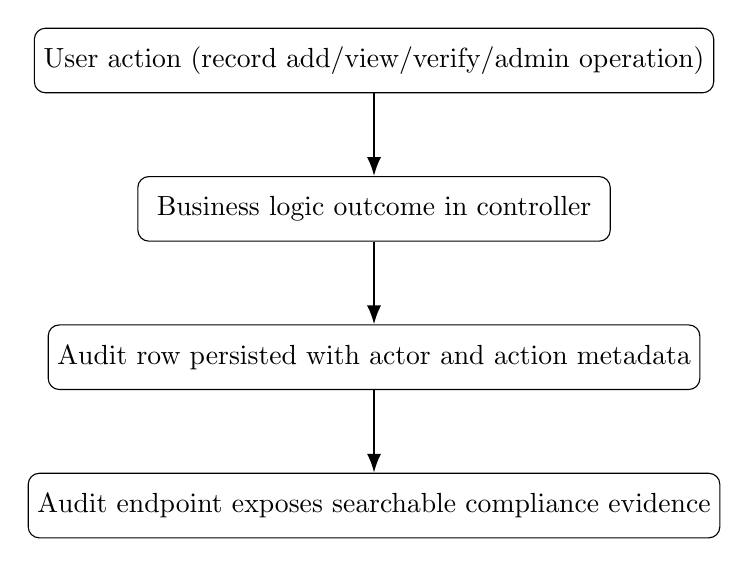
\begin{tikzpicture}[
node distance=1.05cm,
nodebox/.style={draw, rounded corners, align=center, minimum width=6.0cm, minimum height=0.82cm},
arrow/.style={-{Latex[length=2.4mm]}, thick}
]
\node[nodebox] (l1) {User action (record add/view/verify/admin operation)};
\node[nodebox, below=of l1] (l2) {Business logic outcome in controller};
\node[nodebox, below=of l2] (l3) {Audit row persisted with actor and action metadata};
\node[nodebox, below=of l3] (l4) {Audit endpoint exposes searchable compliance evidence};
\draw[arrow] (l1) -- (l2);
\draw[arrow] (l2) -- (l3);
\draw[arrow] (l3) -- (l4);
\end{tikzpicture}
\caption{Audit lifecycle from user action to compliance-visible trace.}
\label{fig:audit-lifecycle}
\end{figure}

\section{Limitations of Current Security Scope}

The current implementation is designed for educational and prototype deployment. It does not claim full production compliance certification and still requires enterprise hardening in key management, immutable remote logging, and regulated governance controls.

\section{Security Enhancement Roadmap}

\begin{enumerate}
\item key rotation and secure vault-backed key lifecycle,
\item optional MFA and stronger password policy enforcement,
\item anomaly alerts for repeated mismatch or suspicious access patterns,
\item periodic signed chain snapshots,
\item administrative security dashboards and audit export pipelines.
\end{enumerate}

\chapter{DEPLOYMENT, TESTING, EVALUATION, AND DISCUSSION}

\section{Deployment Overview}

The project is deployed as a coordinated three-service setup: MySQL database, Express backend API, and React frontend.

\begin{enumerate}
\item Start MySQL (Docker or local instance) and initialize schema.
\item Configure backend environment and run API service.
\item Configure frontend API endpoint and run client service.
\item Validate blockchain status and create a test record.
\item Confirm audit logs and scheduler flows are operational.
\end{enumerate}

This sequence is intentionally ordered to reduce debugging complexity. Database readiness is validated first, then backend service correctness, and finally frontend integration. By enforcing this progression, deployment failures are isolated to a narrower layer and can be corrected quickly during demonstration setup.

\section{Configuration Checklist}

\begin{table}[htbp]
\centering
\caption{Deployment checklist for reproducible setup.}
\label{tab:deployment-checklist}
\begin{tabular}{p{0.34\textwidth} p{0.24\textwidth} p{0.32\textwidth}}
\toprule
\textbf{Item} & \textbf{Required} & \textbf{Verification Method} \\
\midrule
Schema applied to \texttt{healthchain\_db} & Yes & Required tables visible and queryable \\
Backend env configured (.env) & Yes & API boots without runtime config errors \\
Frontend API URL configured & Yes & Login and record retrieval succeed \\
Blockchain file writable & Yes & Block appended after creating a record \\
Audit logging path active & Yes & New entries visible in \texttt{/api/audit-logs} \\
TLS configuration (optional) & Recommended & API/client reachable via HTTPS locally \\
\bottomrule
\end{tabular}
\end{table}

\section{Demo Data and Reset Workflow}

The implementation includes automated demo generation scripts for review readiness:

\begin{enumerate}
\item run schema creation,
\item start backend,
\item run demo generator for doctors/patients/records/appointments,
\item apply seed profile updates,
\item verify blockchain length and sample record integrity.
\end{enumerate}

This workflow ensures repeatable demonstration state before viva or evaluation.

\begin{figure}[H]
\centering
\fbox{\begin{minipage}[c][3.5cm][c]{0.88\textwidth}
\centering
\textbf{Placeholder: Deployment Run Screenshot}\\[0.25cm]
Add: terminal showing backend startup + frontend startup + successful health call.
\end{minipage}}
\caption{Suggested screenshot for Chapter 9: deployment reproducibility evidence.}
\label{fig:placeholder-deployment-run}
\end{figure}

\section{Testing, Evaluation, and Discussion Overview}

After deployment readiness is established, validation moves to behavior correctness and trust verification. The testing scope is not limited to API responses; it also checks role-policy enforcement, deterministic integrity outcomes, scheduler conflict handling, and audit trace visibility. This integrated approach demonstrates that the system is both runnable and reliably verifiable.

\section{Testing Methodology}

Testing was carried out at unit-like function scope, API integration scope, and end-to-end workflow scope to verify that the HealthChain implementation behaves correctly as an engineering system rather than only as a UI demo.

\begin{enumerate}
\item functional API behavior testing,
\item middleware and role enforcement testing,
\item blockchain and tamper-detection testing,
\item scheduler conflict and status-transition testing,
\item audit and observability testing.
\end{enumerate}

\section{Representative Validation Matrix}

\begin{table}[htbp]
\centering
\caption{Representative test/evaluation matrix and outcomes.}
\label{tab:test-cases}
\begin{tabular}{p{0.10\textwidth} p{0.37\textwidth} p{0.20\textwidth} p{0.23\textwidth}}
\toprule
\textbf{ID} & \textbf{Test Case} & \textbf{Expected Result} & \textbf{Observed Result} \\
\midrule
T1 & Valid doctor login & JWT + role claims returned & Passed \\
T2 & Restricted endpoint by wrong role & HTTP 403 Access Denied & Passed \\
T3 & Full SOAP record insert path & Transaction commit + hash + block & Passed \\
T4 & Verify untouched record & SECURE status & Passed \\
T5 & Tamper DB field then verify & TAMPERED status & Passed \\
T6 & Overlapping appointment booking & HTTP 409 conflict & Passed \\
T7 & Audit filter and pagination query & Correct filtered result set & Passed \\
T8 & Chain status validation endpoint & Valid chain in untampered state & Passed \\
\bottomrule
\end{tabular}
\end{table}

\section{Tamper-Evidence Evaluation Scenario}

The critical engineering claim is integrity breach detection. Validation sequence:

\begin{enumerate}
\item create a record through official clinical flow,
\item verify and observe SECURE state,
\item modify stored clinical data directly in DB,
\item re-run verification endpoint,
\item observe TAMPERED verdict.
\end{enumerate}

This confirms independent integrity instrumentation beyond access-control assumptions.

Beyond correctness, this scenario is useful as a communication artifact for external evaluators. It demonstrates that the project can distinguish between normal clinical updates and unauthorized post-write modifications, which is the central trust objective of HealthChain Bridge.

\begin{figure}[H]
\centering
\fbox{\begin{minipage}[c][3.8cm][c]{0.86\textwidth}
\centering
\textbf{Placeholder: Blockchain Verification Evidence Screenshot}\\[0.3cm]
Insert SECURE and TAMPERED verification screenshots before final submission.
\end{minipage}}
\caption{Verification evidence used in testing and evaluation.}
\label{fig:blockchain-verification-evidence}
\end{figure}

\section{Discussion of Results}

\subsection{Positive Outcomes}

\begin{enumerate}
\item modular controllers and middleware produced stable workflow behavior,
\item transactional persistence prevented partial clinical state corruption,
\item blockchain-anchored hashing provided clear tamper evidence,
\item audit logs improved operational accountability and explainability.
\end{enumerate}

\subsection{Observed Engineering Constraints}

\begin{enumerate}
\item file-based ledger is practical but not enterprise-distributed,
\item environment setup consistency strongly affects full harness reliability,
\item current test scope prioritizes functional correctness over load/performance stress.
\end{enumerate}

\subsection{Evaluation Summary}

Overall results indicate that HealthChain Bridge achieves strong academic engineering quality: reproducible workflows, visible integrity checks, and coherent cross-layer integration. The next chapter concludes findings, limitations, and future direction.

\begin{figure}[H]
\centering
\fbox{\begin{minipage}[c][3.5cm][c]{0.88\textwidth}
\centering
\textbf{Placeholder: Clinical Workstation + Blockchain Explorer Screenshots}\\[0.25cm]
Add two images: (1) Clinical Workstation form with live hash preview, (2) Blockchain Explorer showing verified block state.
\end{minipage}}
\caption{Suggested screenshot set for Chapter 9 discussion evidence.}
\label{fig:placeholder-testing-ui-set}
\end{figure}

\chapter{CONCLUSION AND FUTURE ENHANCEMENTS}

\section{Conclusion}

HealthChain Bridge successfully demonstrates how blockchain-backed integrity checks can be integrated into a practical full-stack EHR/Doctor CRM system. The project delivers functional modules for role-based authentication, patient management, SOAP record capture, appointment scheduling, blockchain visualization, and compliance-oriented audit logging.

The key technical contribution is deterministic SHA-256 hashing of structured clinical content and linkage of each record to a chained block. This enables direct detection of unauthorized post-entry modifications while preserving the benefits of normalized relational storage in MySQL.

From an engineering perspective, the project combines frontend usability, backend modularity, transactional persistence, cryptographic integrity, and security-aware middleware in a coherent architecture suitable for final-year academic evaluation.

A strong outcome of the work is that integrity assurance is embedded into normal operational flow rather than treated as a disconnected add-on. Doctors continue using familiar documentation behavior, while the system silently adds verifiable trust instrumentation behind the scenes. This makes the design both technically meaningful and practically adoptable.

\section{Limitations}

Although the system meets its defined goals, several limitations remain:

\begin{enumerate}
\item ledger persistence is file-based and not yet distributed,
\item compliance implementation is educational rather than formally certified,
\item large-scale performance and resilience benchmarks are limited,
\item healthcare interoperability standards are not yet integrated.
\end{enumerate}

\section{Future Scope}

Future versions can extend the platform in both technical and clinical utility dimensions:

\begin{enumerate}
\item migrate blockchain persistence to managed immutable/distributed infrastructure,
\item add digital signatures for clinician-authored records,
\item integrate standards-oriented interoperability gateways,
\item introduce stronger consent policies and governance controls,
\item add monitoring dashboards and anomaly detection pipelines,
\item perform load testing and production hardening,
\item package full deployment with container orchestration and secure CI/CD.
\end{enumerate}

If implemented incrementally, these enhancements can transform the current prototype from strong academic proof-of-concept into a robust pilot-ready platform for integrity-sensitive clinical environments.

\chapter*{REFERENCES}
\addcontentsline{toc}{chapter}{REFERENCES}

\begin{enumerate}
\item S. Nakamoto, ``Bitcoin: A Peer-to-Peer Electronic Cash System,'' 2008.
\item M. Crosby, P. Pattanayak, S. Verma, and V. Kalyanaraman, ``Blockchain Technology: Beyond Bitcoin,'' \textit{Applied Innovation Review}, no. 2, pp. 6--10, 2016.
\item A. Alammary, S. Alhazmi, M. Almasri, and S. Gillani, ``Blockchain-Based Applications in Education: A Systematic Review,'' \textit{Applied Sciences}, vol. 9, no. 12, 2019.
\item A. Roehrs, C. A. da Costa, and R. da Rosa Righi, ``OmniPHR: A Distributed Architecture Model to Integrate Personal Health Records,'' \textit{Journal of Biomedical Informatics}, vol. 71, pp. 70--81, 2017.
\item K. Peterson, R. Deeduvanu, P. Kanjamala, and K. Boles, ``A Blockchain-Based Approach to Health Information Exchange Networks,'' NIST Workshop, 2016.
\item Express.js Documentation, ``Express 5 API Reference.'' [Online]. Available: https://expressjs.com/
\item React Documentation, ``React Developer Reference.'' [Online]. Available: https://react.dev/
\item Node.js Documentation, ``Crypto Module.'' [Online]. Available: https://nodejs.org/api/crypto.html
\item MySQL Documentation, ``MySQL 8.0 Reference Manual.'' [Online]. Available: https://dev.mysql.com/doc/
\item OWASP Foundation, ``JSON Web Token Cheat Sheet.'' [Online]. Available: https://cheatsheetseries.owasp.org/
\end{enumerate}

\appendix
\chapter{SUPPLEMENTARY MATERIALS}

\section{Sample API Payloads}

The following payloads are representative examples used during implementation and validation.

\textbf{A.1 Register Patient Payload}

\begin{verbatim}
POST /api/register
{
  "username": "patient_demo",
  "password": "Demo@123",
  "role": "patient",
  "full_name": "Demo Patient",
  "age": 32,
  "gender": "Female"
}
\end{verbatim}

\textbf{A.2 Create Clinical Record Payload}

\begin{verbatim}
POST /api/records
{
  "patient_id": 5,
  "subjective": "Headache for two days",
  "objective": "Mild fever, BP stable",
  "assessment": "Viral febrile illness",
  "plan": "Paracetamol and hydration",
  "vitals": {
    "temperature": "99.8F",
    "blood_pressure": "120/80",
    "heart_rate": "82"
  }
}
\end{verbatim}

\section{Sample Verification Outputs}

\textbf{A.3 Record Verification Response (Secure)}

\begin{verbatim}
{
  "visit_id": 42,
  "status": "SECURE",
  "db_hash": "f6ac...91e2",
  "chain_hash": "f6ac...91e2"
}
\end{verbatim}

\textbf{A.4 Record Verification Response (Tampered)}

\begin{verbatim}
{
  "visit_id": 42,
  "status": "TAMPERED",
  "db_hash": "73de...2a11",
  "chain_hash": "f6ac...91e2"
}
\end{verbatim}

\section{Sample SQL Tamper Demonstration}

\textbf{A.5 Controlled Tamper Query (For Demonstration Only)}

\begin{verbatim}
UPDATE diagnoses
SET diagnosis_text = 'Modified text for tamper demo'
WHERE visit_id = 42;
\end{verbatim}

This query is executed only in test environments to demonstrate hash mismatch detection.

\section{Optional Screenshot Recommendation}

The report includes a single outcome screenshot in Figure~\ref{fig:blockchain-verification-evidence}.
This evidence image was chosen because it directly demonstrates the blockchain verification capability,
which is the central contribution of the project.

\end{document}
